\documentclass[a4paper]{article}
\usepackage[utf8]{inputenc}
\usepackage[T1]{fontenc}
\usepackage[pdftex]{graphicx}
\usepackage{fancyhdr}
\usepackage{lscape}
\usepackage{color}
\usepackage[english]{babel}
\usepackage{graphicx}
\usepackage[colorinlistoftodos]{todonotes}
\usepackage{listings}
\usepackage{color}
\usepackage{changepage}
\usepackage[margin=1in]{geometry}
\definecolor{codegreen}{rgb}{0,0.6,0}
\definecolor{codegray}{rgb}{0.5,0.5,0.5}
\definecolor{codepurple}{rgb}{0.58,0,0.82}
\definecolor{backcolour}{rgb}{0.95,0.95,0.92}
 
 \lstdefinestyle{mystyle}{
 	backgroundcolor=\color{backcolour},   
 	commentstyle=\color{codegreen},
 	keywordstyle=\color{magenta},
 	numberstyle=\tiny\color{codegray},
 	stringstyle=\color{codepurple},
 	basicstyle=\footnotesize,
 	breakatwhitespace=false,         
 	breaklines=true,                 
 	captionpos=b,                    
 	keepspaces=true,                 
 	numbers=left,                    
 	numbersep=5pt,                  
 	showspaces=false,                
 	showstringspaces=false,
 	showtabs=false,                  
 	tabsize=2
 }
 
\lstset{
	style=mystyle,
	inputencoding=utf8,
	extendedchars=true,
	literate={á}{{\'a}}1 {ã}{{\~a}}1 {é}{{\'e}}1,
	escapechar=\&
}
\title{Algorithmique et structures de données : Mission 2 (produit)}
\date{07 octobre 2014}
\author{Groupe 1.2: Ivan Ahad - Jérôme Bertaux - Rodolphe Cambier \\ 
	Baptiste Degryse - Wojciech Grynczel - Charles Jaquet}



\begin{document}
\maketitle
\paragraph{Question 1}
La profondeur est le nombre de parents qu’un noeud comporte. La racine est donc de profondeur 0, et ses enfants sont de profondeur 1. La hauteur est le nombre maximum de générations en dessous du noeud. Une feuille a une hauteur de 0, et les autre noeuds ont la hauteur de leur enfant le plus haut+1. Le niveau n est l’ensemble des nœuds de profondeur n. Ces notions ne dépendent pas du style d’arbre, elles s'appliquent aux arbres en général car il suffit d’avoir la notion de racine, feuille, enfant et parent pour pouvoir appliquer ces définitions. Ces notions ne dépendent pas de la structure de données utilisée car la représentation ne dépend pas de l’implémentation.

\paragraph{Question 2}

\paragraph{Question 3}

\paragraph{Question 4}

\paragraph{Question 5}

Oui, ce cas peut poser problème pour parcourir l'arbre binaire.

Dans le cas où l'on voudrait, par exemple, parcourir tous les noeuds de l'arbre situés à un même niveau, ne pas avoir la possibilité de remonter peut poser problème et ralentir fortement le processus.

Pour réaliser la méthode parent, on peut faire comme suit: Garder le pointeur sur le noeud dont on veut le parent.
Vérifier si ce noeud n'est pas le root, auquel cas on retourne null.
Parcourir l'arbre noeud par noeud, en vérifiant pour chacun si un de ses fils n'est pas le noeud dont on cherche le parent. 
On finit donc par trouver le parent du noeud de départ.Puisqu'il faut, au pire, parcourir tout l'arbre pour trouver le père, on a une complexité en O(n).

\paragraph{Question 6}

\paragraph{Question 7}

\paragraph{Question 8}
\begin{figure}
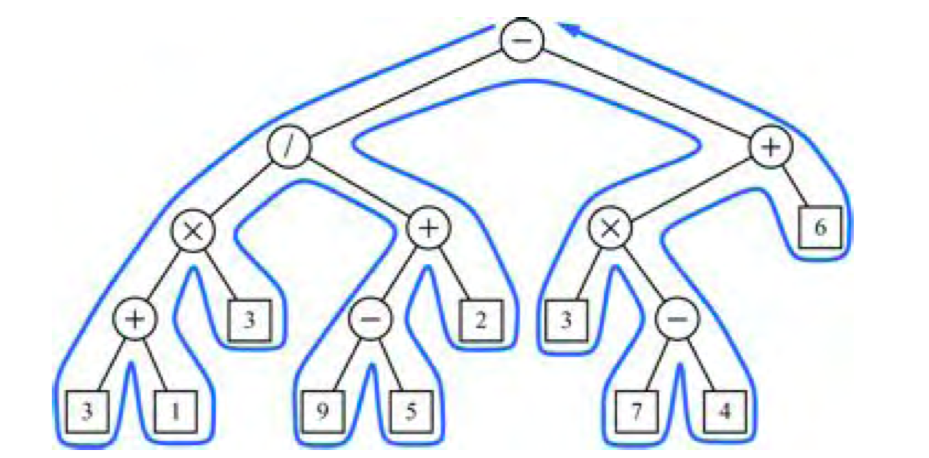
\includegraphics[scale=0.6]{inorder_traversal.png}
\caption{inorder traversal path (from Data Structure And Algorithms in Java p 424)}
\label{inorder}
\end{figure}

C'est le parcours "inorder traversal" d'un arbre binaire qui permet de parcourir l'arbre dans le bon sens. Voir figure \ref{inorder}

\begin{lstlisting}[language=Java]
public String toString(){
if ( T.isExternal(v) )
	return v.getElement().toString();
else
	return "("+ v.left() + v.getElement() + v.right() +")";
}
\end{lstlisting}

\paragraph{Question 9}


\end{document}
